\documentclass[conference]{IEEEtran}
\IEEEoverridecommandlockouts
% The preceding line is only needed to identify funding in the first footnote. If that is unneeded, please comment it out.
\usepackage{cite}
\usepackage{amsmath,amssymb,amsfonts}
\usepackage{algorithmic}
\usepackage{graphicx}
\usepackage{textcomp}
\usepackage{xcolor}
\def\BibTeX{{\rm B\kern-.05em{\sc i\kern-.025em b}\kern-.08em
    T\kern-.1667em\lower.7ex\hbox{E}\kern-.125emX}}
\begin{document}

\title{Rugby Inteligent Camera\\
{\footnotesize \textsuperscript{*}Note: Sub-titles are not captured in Xplore and
should not be used}
\thanks{Identify applicable funding agency here. If none, delete this.}
}

\author{\IEEEauthorblockN{1\textsuperscript{st} Canto da Silva Delatorre, Tiago}
\IEEEauthorblockA{\textit{Electrical and informatics department} \\
\textit{INSA Toulouse}\\
Toulouse, France \\
tcanto-da-si@insa-toulouse.fr}
\and
\IEEEauthorblockN{2\textsuperscript{nd} Given Name Surname}
\IEEEauthorblockA{\textit{dept. name of organization (of Aff.)} \\
\textit{name of organization (of Aff.)}\\
City, Country \\
email address or ORCID}
\and
\IEEEauthorblockN{3\textsuperscript{rd} Given Name Surname}
\IEEEauthorblockA{\textit{dept. name of organization (of Aff.)} \\
\textit{name of organization (of Aff.)}\\
City, Country \\
email address or ORCID}
\and
\IEEEauthorblockN{4\textsuperscript{th} Given Name Surname}
\IEEEauthorblockA{\textit{dept. name of organization (of Aff.)} \\
\textit{name of organization (of Aff.)}\\
City, Country \\
email address or ORCID}
\and
\IEEEauthorblockN{5\textsuperscript{th} Given Name Surname}
\IEEEauthorblockA{\textit{dept. name of organization (of Aff.)} \\
\textit{name of organization (of Aff.)}\\
City, Country \\
email address or ORCID}
\and
\IEEEauthorblockN{6\textsuperscript{th} Given Name Surname}
\IEEEauthorblockA{\textit{dept. name of organization (of Aff.)} \\
\textit{name of organization (of Aff.)}\\
City, Country \\
email address or ORCID}
}

\maketitle

\begin{abstract}
Camera-based tracking systems are increasingly used in sports to enhance performance analysis and broadcast production. However, existing solutions are typically expensive and complex, making them inaccessible for amateur clubs with limited resources. This project aims to develop a cost-effective and functional camera tracking solution to, in real time, broadcast and capture the statistics of an amateur rugby match. Our proposition relies on a multi-camera setup which is controlled by a trained computer vision model, YOLO (You Only Look Once). The conducted tests show an accuracy of 80% in following the match while providing useful statistics through an interactive interface. 
\end{abstract}

\begin{IEEEkeywords}
computer vision, rugby, cost-effective, camera tracking, YOLO
\end{IEEEkeywords}

\section{Introduction}
This document is a model and instructions for \LaTeX.
Please observe the conference page limits. 

\section{Technical choises (explaning how we approched the problem)}

\subsection{Maintaining the Integrity of the Specifications}

The IEEEtran class file is used to format your paper and style the text. All margins, 


\section{Our work}
We can change the order of the project aswell

\subsection{YOLO Model}\label{AA}
To track the focus of a rugby match, we agreed that the most important thing we should track is the ball, but in rugby the ball is small and always hidden between the players or very close to their chest, causing a big problem for the model's identification of the ball. In order to solve this problem, we added the class player; this implies that the players will also be identified by the model.  

In rugby, the teams usually place themselves in lines of attack and defense, so, normally the point of interest will take place where the greatest number of players are. With both classes, we can already create a working tracking model. 

The world of computer vision developers is growing and one of the biggest communities is the Roboflow Universe, which we can find a great number of models and datasets. The project Rugby Detection Computer Vision Model  \cite{b8}  was the closest to our project’s needs, and the pictures used in this dataset are similar to the images we captured in an INSA AS match. 

After testing the model from the project \cite{b8} in some images from the captured match (Fig.~\ref{fig 1} to Fig.~\ref{fig 3}), positive results were achieved: the model responds well to the images, identyfing a big number of player and the ball. Some problems were: confusing the arbitrator with a player, not identifying all the players, and sometimes not seeing the ball.  

\begin{figure}[htbp]
    \centering
    
    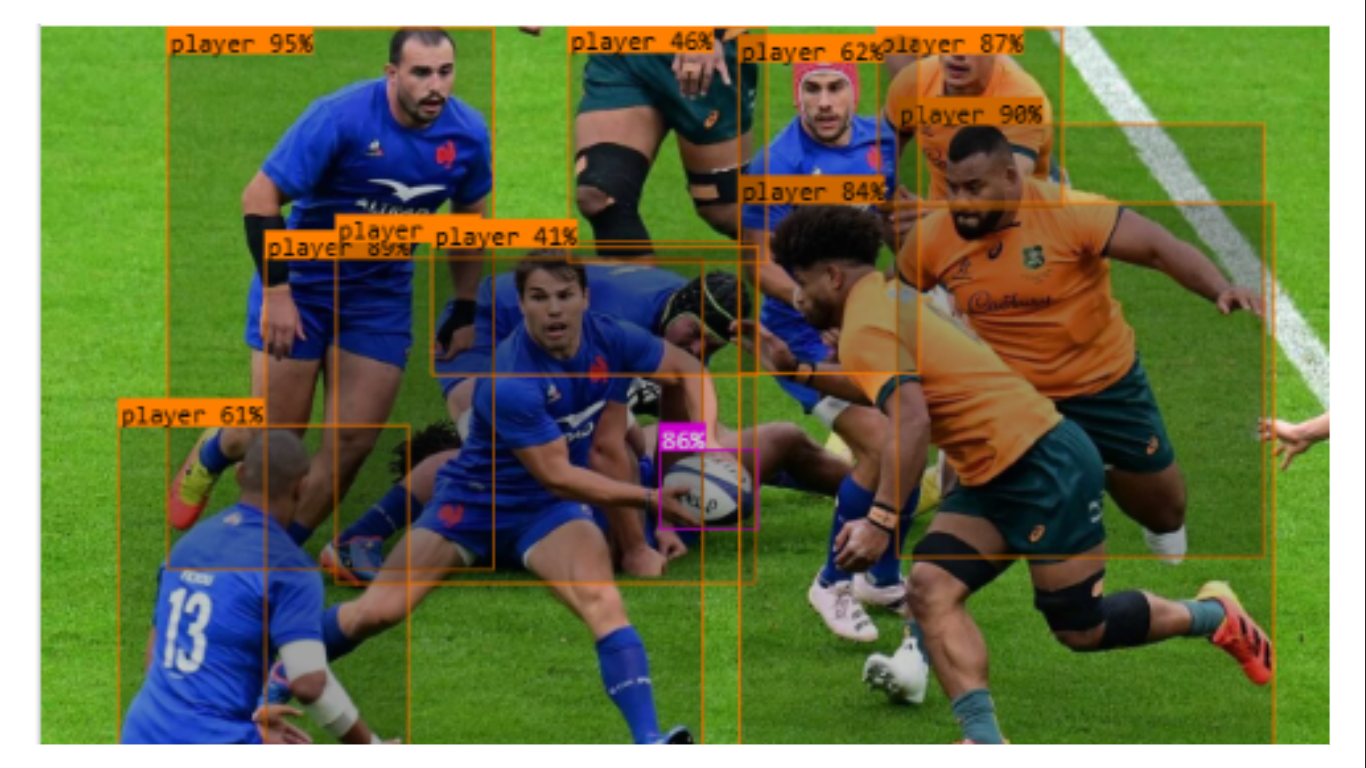
\includegraphics[width=\columnwidth]{Images/img_rugby_1.png}
    \caption{Test image 1, used model from Roboflow\cite{b8}.}
    \label{fig 1}
    
    \vspace{0.5cm} 
    
    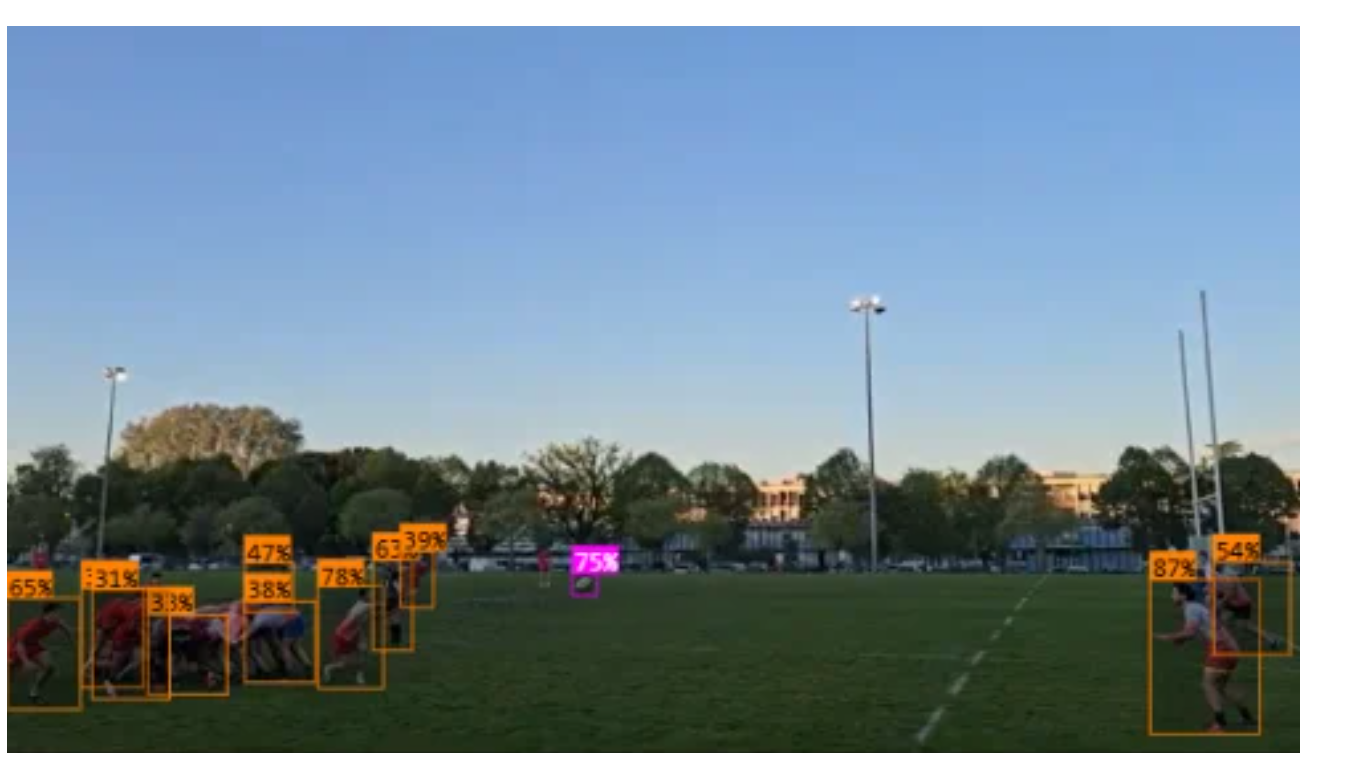
\includegraphics[width=\columnwidth]{Images/img_rugby_2.png}
    \caption{Test image 2, used model from Roboflow\cite{b8}.}
    \label{fig 2}
    
    \vspace{0.5cm}
    
    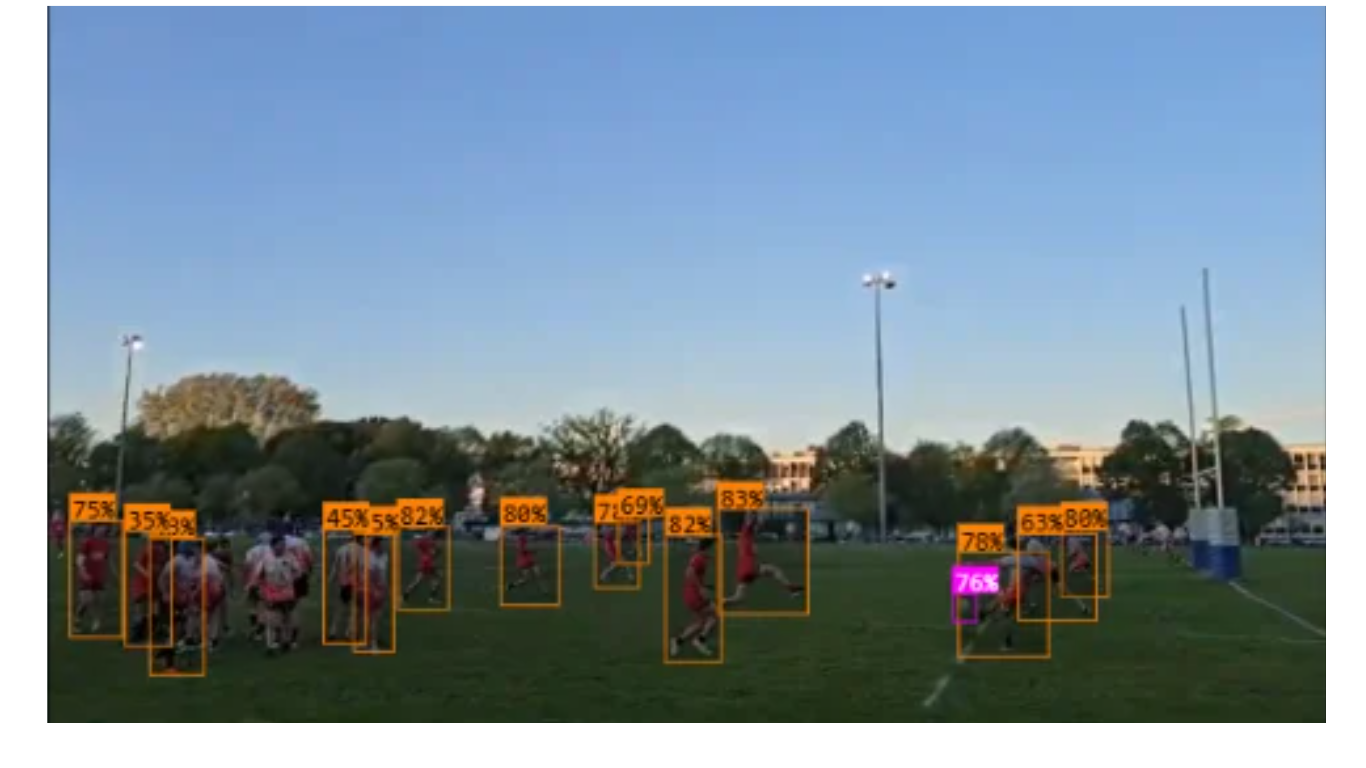
\includegraphics[width=\columnwidth]{Images/img_rugby_3.png}
    \caption{Test image 3, used model from Roboflow\cite{b8}.}
    \label{fig 3}
    
\end{figure}



Unfortunately, the model \cite{b8} isn’t accessible to download, so it wouldn’t  be possible to use in a real time application, because for every frame the Roboflow repository would have to be accessed on the internet, increasing the cost and delay of the image processing. 

To solve the presented problem, the project’s dataset \cite{b8} was cloned and a new AI model was trained, hoping to achieve the same results as the previous. Four models were created, two with yolov8n, one with yolov8s and the last with yolov8m; they were all tested in an image not from the dataset [??? Show images of the test??? ].  

These models aren’t as good as the previous one, but they are functional for video analyses and can be used for real-time applications.  

IMAGES COMPARISON 

To validate our models, we tested it in a video of an INSA AS match, but the power of the available GPU wasn’t enough to analyze a nineteen second video (with 1141 frames). So, we couldn’t validate our models in a hole video but, analyzing in a smaller video, we can see some problems of players and ball identification, showing how the project would look like in a real-time solution. 

Regarding the YOLO model we can conclude that this solution works for identification of our needs to choose the best camera but, trying to find a low-cost solution for the amateur clubs we arrived at a lack of computing power that probably will increase the cost of this approach.  

To improve this project, we plan on using another YOLO model\cite{b9} to see the statistics of the game as well, identifying tackle, penalty kick, throw-in, scrum, and other similar rugby situations that our other model can’t identify. Another aimed improvement is to create a system\cite{b9} so the model could be able to after identifying the players, separate them between team A and team B. The system consists of a Sigmoid loss language image pre-trained\cite{b9} (extract color information from the player’s shirt), associated with an UMAP\cite{b9} (compact the previous information) and a Kmeans \cite{b9} (sort both teams). These improvements would highly increase the quality of the performance analysis of the teams. 

\subsection{Video Positioning teams part}
\begin{itemize}
\item Use either SI (MKS) or CGS as primary units. (SI units are encouraged.) English units may be used as secondary units (in parentheses). An exception would be the use of English units as identifiers in trade, such as ``3.5-inch disk drive''.
\end{itemize}

\subsection{Video Acquisition and Transmission Architecture}
Real-time automated tracking of rugby players imposes strict constraints regarding bandwidth, latency, and hardware costs. This section details the technological choices made to ensure a fluid and synchronized video stream to the central processing unit.
\subsection{Capture Device Choice}
Several capture solutions were evaluated to meet the requirements of the multi-camera tracking project. The use of cameras on motorized platforms was initially considered for its dynamic tracking capability—which could have reduced the number of cameras needed and thus the total cost. However, extreme sensitivity to control delays and prohibitive costs led to its rejection. Similarly, solutions based on microcontrollers such as Arduino, while inexpensive, offered insufficient acquisition performance and resolution for exploitation via YOLOv8 detection models.

Ultimately, smartphones were selected as the capture units. These devices offer an optimal compromise:
\begin{itemize}[label=\textbullet]
    \item \textbf{Image Quality :} High-resolution sensors capable of providing stable streams.
    \item \textbf{Cost :} Utilization of existing hardware, drastically reducing the initial investment.
    \item \textbf{Wireless Capability :} 
\end{itemize}

\section{3.2 \quad Evaluation of Streaming Protocols}
 
To route the video streams from the smartphones to the processing computer, three main
protocols were compared:
 

\vspace{0.5em}
\begin{center}
\renewcommand{\arraystretch}{1.2}
\begin{tabular}{|p{1.6cm}|p{1.5cm}|p{1.1cm}|p{2.6cm}|}
    \hline
    \textbf{Protocol} & \textbf{Infra-structure} & \textbf{Latency} & \textbf{Stability / Cost} \\
    \hline
    SRT & 4G / 5G & Low & Excellent; high subscription costs \\
    \hline
    RTMP & 4G/5G + remote server & Medium & Industry standard (Youtube, Twitch); requires a server \\
    \hline
    HTTP (Local) & Wi-Fi (router) & \textbf{Optimal} & Excellent stability; no recurring cost \\
    \hline
\end{tabular}
\end{center}
\vspace{0.5em}
 


The \textbf{HTTP protocol over a local network} was selected. Unlike cellular solutions
(SRT/RTMP) that depend on public network load and incur data costs, the local network
allows full control, high stability, and minimizes latency.
 
%-----------------------------------------------------------
\section{3.3 \quad Local Network Implementation and Topology}
 
The network architecture put in place relies on the creation of a \textbf{high-performance
private Wi-Fi network} (using a HUAWEI WiFi AX3-type router). This configuration makes it
possible to avoid potential interference with the public networks of stadiums.
 
The system is structured as follows:
 
\begin{enumerate}[leftmargin=2em]
    \item \textbf{Wireless transmission:} The four smartphones transmit their respective
          streams to the central access point via the HTTP protocol. Tests in real conditions
          validated an effective range of \textbf{80 metres}, covering a significant portion
          of the playing surface.
 
    \item \textbf{Downstream link:} The router is connected to the processing computer
          (YOLOv8 computing unit) via a gigabit Ethernet connection. This wired link
          ensures that the bottleneck does not occur at the final data reception stage.
 
    \item \textbf{Centralised processing:} The computer simultaneously receives the four
          streams to perform player detection and tracking, enabling a precise spatial
          reconstruction of the game action.
\end{enumerate}
 
% Placeholder for real test photo
\begin{figure}[h]
   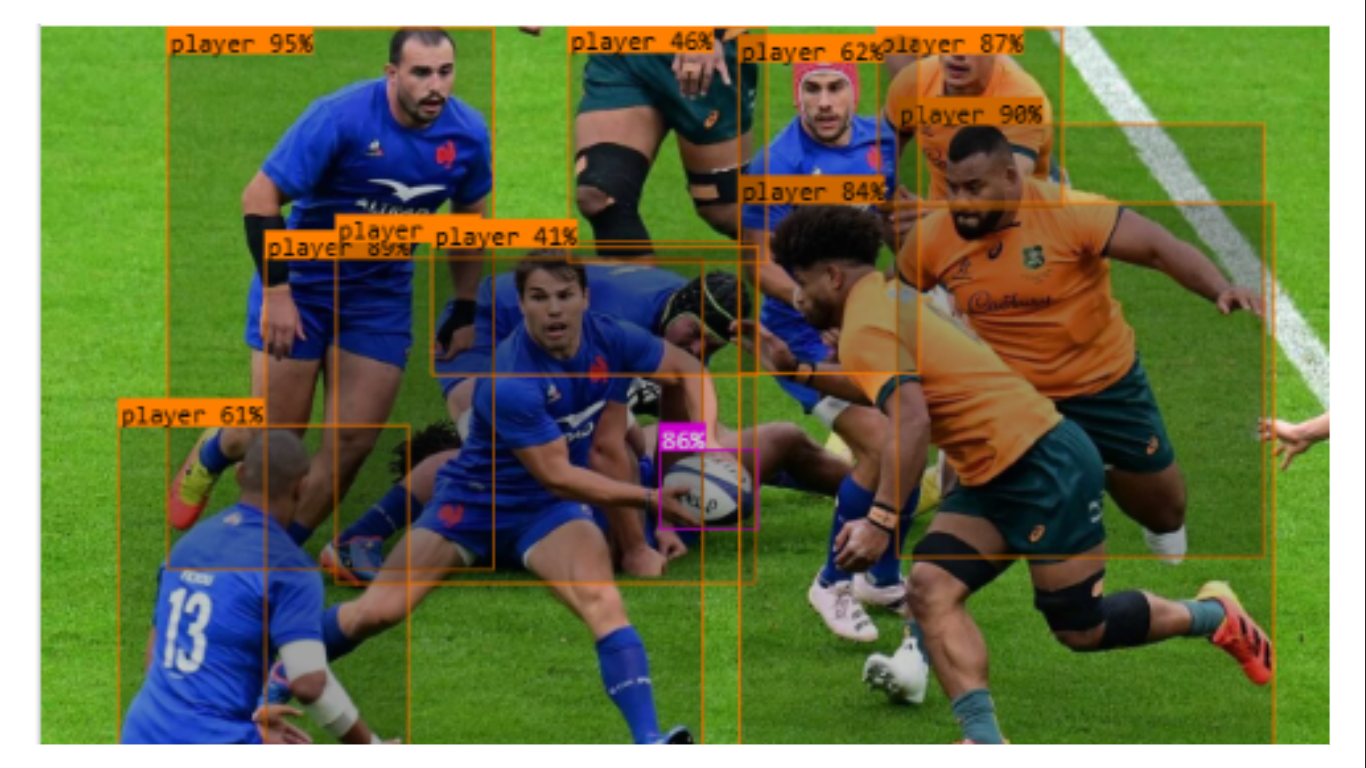
\includegraphics[width=\columnwidth]{Images/img_rugby_1.png}
    \caption{Network topology: four smartphones transmit wirelessly via HTTP (80\,m range)
             to a private Wi-Fi router, which forwards data via gigabit Ethernet to the
             YOLOv8 processing computer.}
    \label{fig 4}
\end{figure}
 

\subsection{Camera score algorithim}

Please use ``soft'' (e.g., \verb|\eqref{Eq}|) cross references instead

\subsection{IHM}\label{SCM}
\begin{itemize}
\item The word ``data'' is plural, not singular.
\end{itemize}
An excellent style manual for science writers is \cite{b7}.

\subsection{Authors and Affiliations}
\textbf{The class file is designed for, but not limited to, six authors.} A 
minimum of one author is required for all conference articles. Author names 
should be listed starting from left to right and then moving down to the 
next line. This is the author sequence that will be used in future citations 
and by indexing services. Names should not be listed in columns nor group by 
affiliation. Please keep your affiliations as succinct as possible (for 
example, do not differentiate among departments of the same organization).

\subsection{Identify the Headings}
Headings, or heads, are organizational devices that guide the reader through 
your paper. There are two types: component heads and text heads.

Component heads identify the different components of your paper and are not 
topically subordinate to each other. Examples include Acknowledgments and 
References and, for these, the correct style to use is ``Heading 5''. Use 
``figure caption'' for your Figure captions, and ``table head'' for your 
table title. Run-in heads, such as ``Abstract'', will require you to apply a 
style (in this case, italic) in addition to the style provided by the drop 
down menu to differentiate the head from the text.

Text heads organize the topics on a relational, hierarchical basis. For 
example, the paper title is the primary text head because all subsequent 
material relates and elaborates on this one topic. If there are two or more 
sub-topics, the next level head (uppercase Roman numerals) should be used 
and, conversely, if there are not at least two sub-topics, then no subheads 
should be introduced.

\subsection{Figures and Tables}
\paragraph{Positioning Figures and Tables} Place figures and tables at the top and 
bottom of columns. Avoid placing them in the middle of columns. Large 
figures and tables may span across both columns. Figure captions should be 
below the figures; table heads should appear above the tables. Insert 
figures and tables after they are cited in the text. Use the abbreviation 
``Fig.~\ref{fig}'', even at the beginning of a sentence.

\begin{table}[htbp]
\caption{Table Type Styles}
\begin{center}
\begin{tabular}{|c|c|c|c|}
\hline
\textbf{Table}&\multicolumn{3}{|c|}{\textbf{Table Column Head}} \\
\cline{2-4} 
\textbf{Head} & \textbf{\textit{Table column subhead}}& \textbf{\textit{Subhead}}& \textbf{\textit{Subhead}} \\
\hline
copy& More table copy$^{\mathrm{a}}$& &  \\
\hline
\multicolumn{4}{l}{$^{\mathrm{a}}$Sample of a Table footnote.}
\end{tabular}
\label{tab1}
\end{center}
\end{table}

\begin{figure}[htbp]
\centerline{
\includegraphics{Conference-LaTeX-template_10-17-19/fig1.png}}
\caption{Example of a figure caption.}
\label{fig}
\end{figure}

Figure Labels: Use 8 point Times New Roman for Figure labels. Use words 
rather than symbols or abbreviations when writing Figure axis labels to 
avoid confusing the reader. As an example, write the quantity 
``Magnetization'', or ``Magnetization, M'', not just ``M''. If including 
units in the label, present them within parentheses. Do not label axes only 
with units. In the example, write ``Magnetization (A/m)'' or ``Magnetization 
\{A[m(1)]\}'', not just ``A/m''. Do not label axes with a ratio of 
quantities and units. For example, write ``Temperature (K)'', not 
``Temperature/K''.

\section*{Acknowledgment}

The preferred spelling of the word ``acknowledgment'' in America is without 
an ``e'' after the ``g''. Avoid the stilted expression ``one of us (R. B. 
G.) thanks $\ldots$''. Instead, try ``R. B. G. thanks$\ldots$''. Put sponsor 
acknowledgments in the unnumbered footnote on the first page.

\section*{References}

Please number citations consecutively within brackets \cite{b1}. The 
sentence punctuation follows the bracket \cite{b2}. Refer simply to the reference 
number, as in \cite{b3}---do not use ``Ref. \cite{b3}'' or ``reference \cite{b3}'' except at 
the beginning of a sentence: ``Reference \cite{b3} was the first $\ldots$''

Number footnotes separately in superscripts. Place the actual footnote at 
the bottom of the column in which it was cited. Do not put footnotes in the 
abstract or reference list. Use letters for table footnotes.

Unless there are six authors or more give all authors' names; do not use 
``et al.''. Papers that have not been published, even if they have been 
submitted for publication, should be cited as ``unpublished'' \cite{b4}. Papers 
that have been accepted for publication should be cited as ``in press'' \cite{b5}. 
Capitalize only the first word in a paper title, except for proper nouns and 
element symbols.

For papers published in translation journals, please give the English 
citation first, followed by the original foreign-language citation \cite{b6}.

\begin{thebibliography}{00}
\bibitem{b1} G. Eason, B. Noble, and I. N. Sneddon, ``On certain integrals of Lipschitz-Hankel type involving products of Bessel functions,'' Phil. Trans. Roy. Soc. London, vol. A247, pp. 529--551, April 1955.
\bibitem{b2} J. Clerk Maxwell, A Treatise on Electricity and Magnetism, 3rd ed., vol. 2. Oxford: Clarendon, 1892, pp.68--73.
\bibitem{b3} I. S. Jacobs and C. P. Bean, ``Fine particles, thin films and exchange anisotropy,'' in Magnetism, vol. III, G. T. Rado and H. Suhl, Eds. New York: Academic, 1963, pp. 271--350.
\bibitem{b4} K. Elissa, ``Title of paper if known,'' unpublished.
\bibitem{b5} R. Nicole, ``Title of paper with only first word capitalized,'' J. Name Stand. Abbrev., in press.
\bibitem{b6} Y. Yorozu, M. Hirano, K. Oka, and Y. Tagawa, ``Electron spectroscopy studies on magneto-optical media and plastic substrate interface,'' IEEE Transl. J. Magn. Japan, vol. 2, pp. 740--741, August 1987 [Digests 9th Annual Conf. Magnetics Japan, p. 301, 1982].
\bibitem{b7} M. Young, The Technical Writer's Handbook. Mill Valley, CA: University Science, 1989.
\bibitem{b8} Roboflow Universe public project made by Rugby Ruck. ''Rugby Detection Computer Vision Model''. https://universe.roboflow.com/rugby-ruck/rugby-detection-m0wvs . Accessed: 17 April 2026.
\bibitem{b9} Roboflow.''Football AI Tutorial: From Basics to Advanced Stats with Python''. 22 August 2024. Accessed: April 2026. Available: https://www.youtube.com/watch?v=aBVGKoNZQUw
\end{thebibliography}
\vspace{12pt}
\color{red}
IEEE conference templates contain guidance text for composing and formatting conference papers. Please ensure that all template text is removed from your conference paper prior to submission to the conference. Failure to remove the template text from your paper may result in your paper not being published.

\end{document}
